\documentclass[../main.tex]{subfiles}
\usepackage{silence}
\WarningFilter{glossaries}{No \printglossary or \printglossaries found}
\robExtConfigure{disable externalization}
\begin{document}
\ifSubfilesClassLoaded{%
	\graphicspath{{figures/7-Interpretability/}}%
	\setcounter{chapter}{6}%
}{
	\graphicspath{{../figures/7-Interpretability/}}%
}
\chapter{Explain with counterfactuals}\label{chap:counterfactuals}
\minitocpage
\section{Methods}
	main introduction to our arch
	robust model = adversarial training
	\subsection{\glsfmtshortpl{gan} to generate counterfactuals}
		\begin{figure}[htbp]
			\centering
			\begin{tikzpicture}[inner sep=0pt, very thick]
				\node at (0,0) [square, draw, minimum size=1.5cm] (xin) {\(x\)};
				\node (gen) [right=1cm of xin.east, anchor=west, rounded rectangle, rounded rectangle west arc=none, draw, minimum height=1cm, minimum width=11mm] {\(G\)};
				\node (delta) [right=1.5cm of gen.east, anchor=west,square, draw, minimum size=1.5cm] {\(\delta\)};
				\node (add) [right=5mm of delta.east, anchor=west, draw, circle, minimum size=7.5mm] {};
				\draw (add.north) -- (add.south);
				\draw (add.west) -- (add.east);
				\node (xcf) [right=5mm of add.east, anchor=west,square, draw, minimum size=1.5cm] {\(x^{\text{CF}}\)};
				\node (cl1) [right=1cm of xcf.east, anchor=west, rounded rectangle, rounded rectangle west arc=none, draw, minimum height=1cm, minimum width=11mm] {\(\operatorname{Cl}\)};
				\node (cly) [right=6mm of cl1.east, anchor=west] {\(\hat{y}\)};
				\node (ycf) [right=1.5cm of cly.east, anchor=west] {\(y^{\text{CF}}\)};

				\node (dis) [below=7mm of cl1.south, anchor=north, rounded rectangle, rounded rectangle west arc=none, draw, minimum height=1cm, minimum width=11mm] {\(D\)};
				\node (realfake) at (dis.east -| cly.south)  {\(s\)};
				\node[align=left] (labelrealfake) at (realfake.east -| ycf.south) {0 \\ 1};

				\node (cl2) [above=7mm of cl1.north, anchor=south, rounded rectangle, rounded rectangle west arc=none, draw, minimum height=1cm, minimum width=11mm] {\(\operatorname{Cl}_{T}\)};
				\node (cl2y) at (cl2.east -| cly.north)  {\(\hat{y}_{T}\)};
				\node (ytissue) at (cl2y.east -| ycf.north) {\(y_{T}\)};

				\node (xreal) at (xcf.south |- dis.east) [draw, square, minimum size=1.5cm, double copy shadow={shadow xshift=-.5ex, shadow yshift=.5ex, opacity=.5}, fill=white] {\(\symcal{X}\)};

				\draw[-stealth] (xin.east) -- (gen.west);
				\draw[-stealth] (gen.east) -- node [midway, matrix, draw=none, anchor=center, yshift=0.7em] {
					\node[draw=none,minimum size=1.2em] {\(\symcal{M}\)}; \\
					\node[draw,fill=black,minimum size=1.2em] {};  \\
					\node[draw,fill=white,minimum size=1.2em] {};  \\
					\node[draw,fill=black,minimum size=1.2em] {};  \\
					\node[draw,fill=white,minimum size=1.2em] {};  \\
					\node[draw,fill=black,minimum size=1.2em] {};  \\
					\node[draw,fill=white,minimum size=1.2em] {};  \\
				} (delta.west);
				\draw[-stealth] (delta.east) -- (add.west);
				\draw[-stealth]  (xin.south) -- ++(0,-12mm) -| (add.south);
				\draw[-stealth] (add.east) -- (xcf.west);
				\draw[-stealth] (xcf.east) -- (cl1.west);
				\draw[-stealth] (xcf.east) -- ++(4mm, 0) |- ([yshift=2mm]dis.west);
				\draw[-stealth] ([yshift=-2mm]xreal.east) -- ([yshift=-2mm]dis.west);
				\draw[-stealth] (xcf.east) -- ++(4mm, 0) |- (cl2.west);
				\draw[-stealth] (cl1.east) -- (cly.west);
				\draw[-stealth] (cl2.east) -- (cl2y.west);
				\draw[-stealth] (dis.east) -- (realfake.west);
				\draw[stealth-stealth, dashed] (cly.east) -- node [midway,above, yshift=0.5ex] {\(\symcal{L}_{\text{CE}}\)}  (ycf.west);
				\draw[stealth-stealth, dashed] (cl2y.east) -- node [midway,above, yshift=0.5ex] {\(\symcal{L}_{\text{CE}}\)}  (ytissue.west);
				\draw[stealth-stealth, dashed] (realfake.east) -- node [midway,above, yshift=0.5ex] {\(\symcal{L}_{\text{GAN}}\)}  (labelrealfake.west);
			\end{tikzpicture}
			\caption[Architecture of the counterfactual \glsfmtshort{gan}]{Architecture of the counterfactual \glsfmtshort{gan}. The example \(x\), for which a counterfactual is searched, is passed through the generator \(G\) to obtain the optimal perturbation \(\delta\). This perturbation is added to the input to obtain the counterfactual point \(x^{\text{CF}}\). During the training phase, the counterfactual point is evaluated with two classifiers to ensure the point is classified to the desired class (\(\operatorname{Cl}\)) and belongs to the same tissue as the original point (\(\operatorname{Cl}_{T}\)). A critic \(D\) is used to ensure the generated point belongs to the original data distribution. }\label{fig:gan_cf}
		\end{figure}
		remind the three main properties of counterfactual point
		Sparsity: \(\left\|\delta\right\|_{1}\)
		Actionnability: masking the output of \(G\) with \(\symcal{M}\)
		Data manifold closeness: \(G\)

		Details on the training strategy WGAN-GP
	\subsection{Counterfactuals evaluation}
		distance, L0 to check the sparsity
		A realistic counterfactual should have points in its neighborhood that are classified the same.
		yNN proportion of point in the k nearest neighbors classified the same accuracy based on the kNN neighbors characterization \cite{Carla_CF}
		can also be visualized by projecting counterfactuals points onto the UMAP space obtained from the training data.
		Sucess rate / Accuracy are we able to change the label for all points
		UMAP evaluation + neighbors characterization

	\subsection{Getting a robust model: adversarial training}
		adversarial and counterfactuals close proximity (solve similar optimization problem).
		Prevent the GAN from finding adversarial --> make the classifier robust to adversarial examples
		achieved with adversarial training: opt problem
		algo

	\subsection{Adversarial Metrics}
		To evaluate model robustness, we used three metrics: model smoothness, margin decision~\cite{MarginDecision} and boundary thickness.
		The details of each metric is given below:
		\begin{description}[
				style=multiline,
				leftmargin=!,
				labelwidth=2.5cm
			]
			\item[Model smoothness]
				insensitiveness of the output to the input perturbation~\cite{MarginDecision}
				KL divergence
				smaller smoothness is better
			\item[Margin decision]
				This metric measure the distance of an example to the decision boundary~\cite{MarginDecision}.
				text version of the metric
				\begin{equation}
					g\left(\symbf{x}\right)_{y} - \max_{i \neq y} g\left(\symbf{x}\right)_{i}
				\end{equation}
				A higher margin decision is better.
			\item[Boundary thickness]
				Thick decision boundaries lead to improved performance
				thicker boundary helps improve robustness against adversarial examples
				\begin{equation}
					\left\|x - x^{\star}\right\|_{2} \int_{0}^{1} \symbb{1}\left\{ \alpha < g_{ij}\left(tx + \left(1-t\right)x^{\star} \right) < \beta\right\}
				\end{equation}
		\end{description}


\section{Preliminary results}
	\subsection{Adversarial study}
		what attacks we used PGD Linf cite package
		how did we choose epsilon (distance class)
		BN problems, consider models without batch normalization
		comparison of different models, justification problem BatchNorm
		present the different models
		identify the optimal number of training steps for each model
		compare different epsilon attacks
		targeted vs untargeted
		Metrics
		neighbors characterization
		\begin{figure}[htbp]
			\centering
			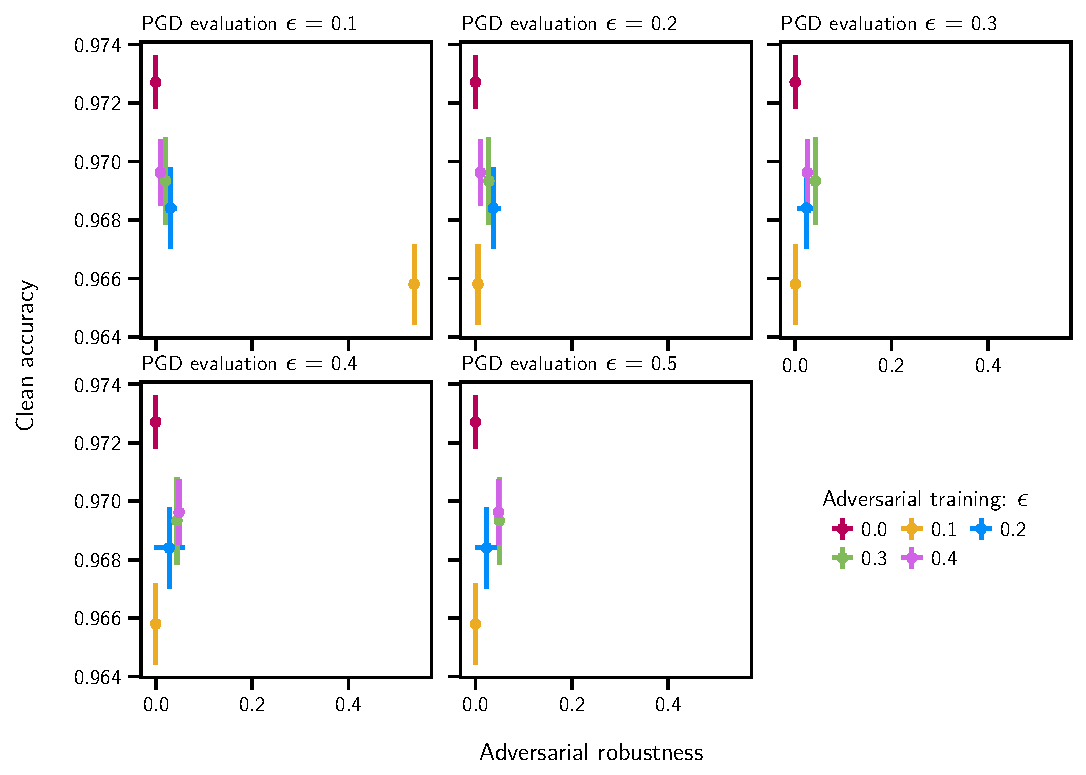
\includegraphics{MLP_BN_adversarial_tradeoff.pdf}
			\caption{MLP with BatchNorm adversarial tradeoff}\label{fig:mlp_bn_adv_tradeoff}
		\end{figure}

		\begin{figure}[htbp]
			\centering
			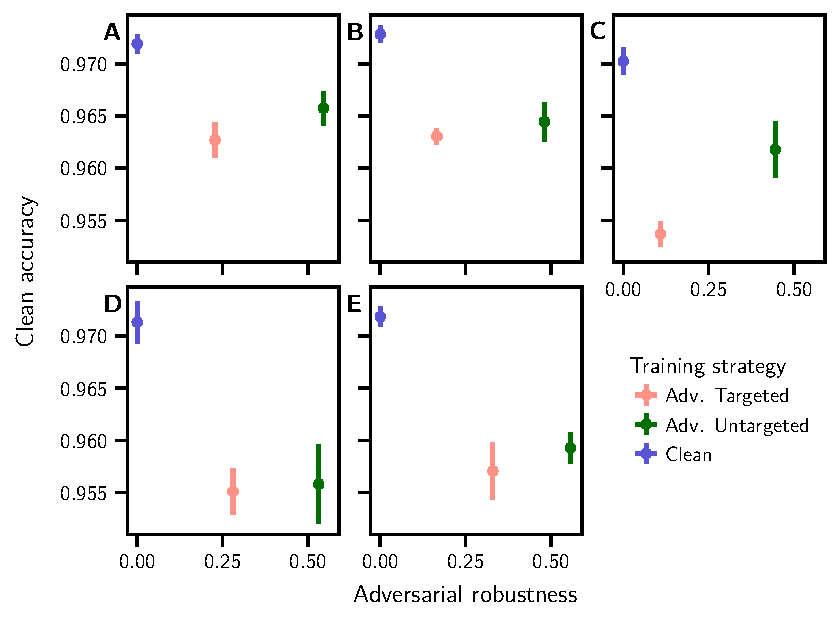
\includegraphics{adversarial_robustness_strategy.pdf}
			\caption{Adversarial robustness strategy}\label{fig:adv_robust_strat}
		\end{figure}

		\begin{landscape}
			\begin{figure}[htbp]
				\centering
				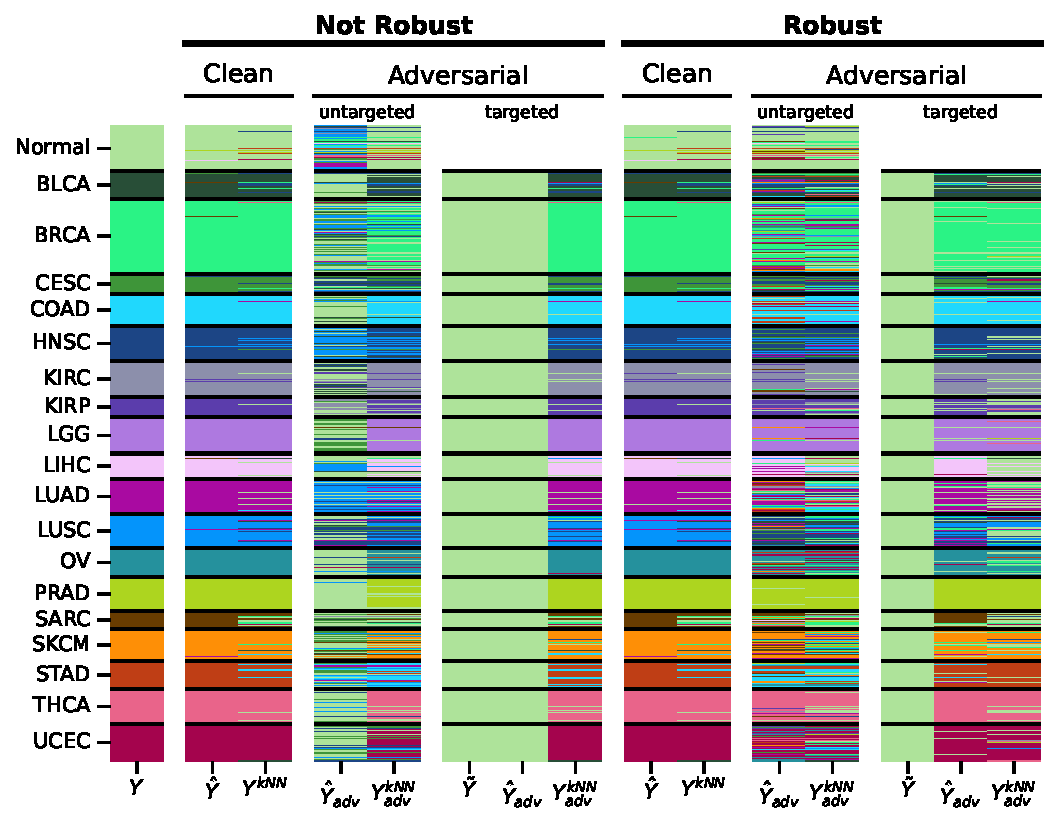
\includegraphics{MLP_BN_knn_comparison.pdf}
				\caption{MLP BatchNorm knn comparison}\label{fig:mlp_bn_knn_comp}
			\end{figure}
		\end{landscape}

		\cite{SzegedyZSBEGF13}
		\begin{table}[htbp]
			\sisetup{round-mode=places,round-precision=2}
			\caption[Adversarial metrics]{Some LEGEND, a robust model corresponds to a model that have been adversarially trained.}\label{tab:metrics_adv}
			\csvreader[
				no head,
				centered tabularray={%
						colspec={%
								Q[c,m]
								Q[si={table-format=2.2,table-number-alignment=center}, wd=1.4cm]%
								Q[si={table-format=2.2,table-number-alignment=center}, wd=1.4cm]%
								Q[si={table-format=2.2,table-number-alignment=center}, wd=1.4cm]%
								Q[si={table-format=2.2,table-number-alignment=center}, wd=1.4cm]%
								Q[si={table-format=2.2,table-number-alignment=center}, wd=1.6cm]%
								Q[si={table-format=2.2,table-number-alignment=center}, wd=1.6cm]%
							},%
						row{1-2} = {guard},
						row{2} = {c,m},
						row{3-Z} = {font=\small},
						row{1} = {font=\bfseries},
						cell{1}{2} = {r=1,c=2}{c, wd=2.8cm},
						cell{1}{4} = {r=1,c=2}{c, wd=2.8cm},
						cell{1}{6} = {r=1,c=2}{c, wd=3.2cm},
						hline{1} = {2-Z}{2pt},%
						hline{Z} = {2pt},%
						hline{2-3} = {1pt},%
						column{even} = {rightsep=2pt},
						column{odd[3-Z]} = {leftsep=2pt},
						cell{3-Z}{1} = {font=\normalsize}
					}
			]{%
				\ifSubfilesClassLoaded{%
					data/AdversarialMetrics.csv%
				}{%
					../data/AdversarialMetrics.csv%
				}%
			}{}{\csvlinetotablerow}
		\end{table}
	\subsection{Counterfactuals}








		counterfactuals, could we compare the proposed treatments with, when available, the treatment scheme of the patient.

\end{document}
